\chapter{Related Work}
We situate our approach within prior art on fundus disease classification, attention mechanisms for CNNs, and ODIR\textendash 5K research. We first outline CNN baselines and transfer learning practice for fundus imaging, then summarize channel/spatial attention (SE, CBAM, ECA) and token self\textendash attention (ViT/DeiT), and finally review ODIR\textendash 5K labeling practices and recent state of the art.
\section{Fundus Image Classification}
CNNs such as VGG, ResNet, and EfficientNet have been widely applied to fundus image analysis for diabetic retinopathy screening and broader ocular disease classification. EfficientNet family models leverage compound scaling and strong ImageNet pretraining for competitive performance at modest compute cost \cite{tan2019efficientnet}.

Recent practitioner work on Kaggle explores end\textendash to\textendash end pipelines for eye disease classification, e.g., \cite{waleedKaggleEyes}, illustrating common preprocessing, transfer learning backbones, and evaluation practices that complement academic baselines.

\section{Attention Mechanisms}
Channel and spatial attention mechanisms (SE, CBAM, ECA) improve CNN feature quality by adaptively reweighting salient signals. CBAM applies sequential channel and spatial attention via lightweight modules with minimal overhead \cite{woo2018cbam}. For accessible primers on CBAM and related attention modules, see \cite{cbamMedium, cbamDO}. Vision transformers (ViT) and token\textendash based self\textendash attention have also shown promise, but often require larger datasets or heavy augmentation.

\begin{figure}[t]
  \centering
  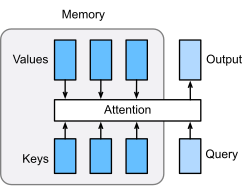
\includegraphics[width=0.92\textwidth]{../new_work/websites/Attention (machine learning) - Wikipedia_files/Attention_mechanism_overview.svg.png}
  \caption{Overview of attention mechanisms (adapted from Wikipedia \cite{wikiAttention}): queries, keys, and values produce attention weights to focus computation on salient content. We use convolutional attention (CBAM) rather than token attention (ViT) to keep the inductive biases of CNNs for fundus images.}
  \label{fig:attn_overview_wiki}
\end{figure}

\begin{figure}[t]
  \centering
  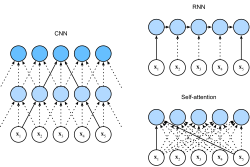
\includegraphics[width=0.9\textwidth]{../new_work/websites/Attention (machine learning) - Wikipedia_files/Self-attention_in_CNN,_RNN,_and_self-attention.svg.png}
  \caption{Self\textendash attention styles across architectures (Wikipedia \cite{wikiAttention}). Our approach augments a CNN with CBAM, which performs channel and spatial attention on feature maps instead of sequence tokens.}
  \label{fig:self_attn_styles}
\end{figure}

\begin{figure}[t]
  \centering
  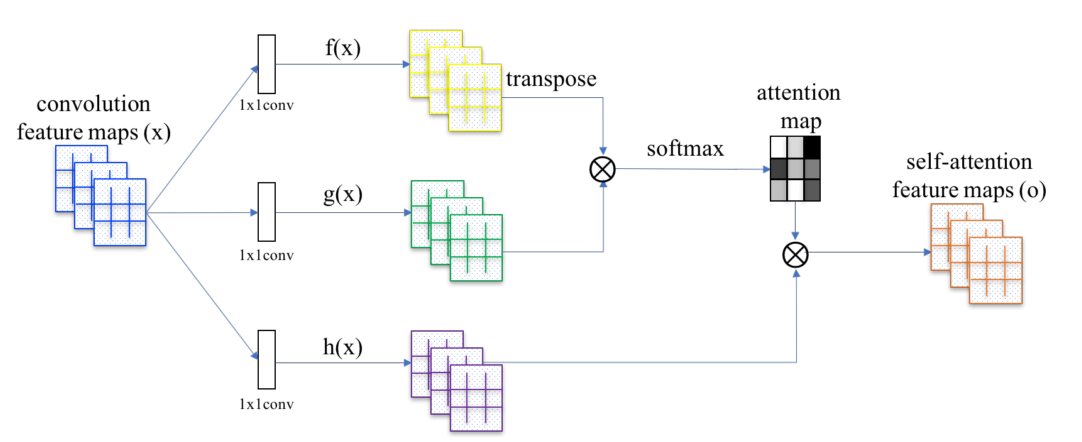
\includegraphics[width=0.95\textwidth]{../new_work/websites/Attention Mechanisms in Computer Vision_ CBAM _ DigitalOcean_files/main_model.png}
  \caption{CBAM concept illustration (DigitalOcean tutorial \cite{cbamDO}): channel attention (what) followed by spatial attention (where). We adopt this sequential design in our EfficientNet+CBAM model.}
  \label{fig:cbam_do_model}
\end{figure}

\subsection{From SE to CBAM, BAM, and ECA}
Squeeze\textendash and\textendash Excitation (SE) \cite{hu2018squeeze} introduced channel reweighting via global pooling and a bottleneck MLP, greatly improving many CNN backbones. BAM \cite{park2018bam} adds a parallel attention branch with dilated convolutions to enlarge receptive fields, while ECA \cite{wang2020eca} removes the MLP in favor of local cross\textendash channel interactions using 1D convolutions. CBAM \cite{woo2018cbam} extends SE by combining channel and spatial attention sequentially, capturing both what and where to attend.

\subsection{Attention in Medical Imaging}
In medical CV tasks, data scarcity and domain shift often favor CNNs with lightweight attention over pure transformers. Channel/spatial attention has benefited retinal disease grading, lesion localization, and OCT segmentation by enhancing salient structures (discs, vessels, macula). Our EfficientNet+CBAM results on ODIR\textendash 5K align with this trend: small overhead, improved per\textendash class recall, and clearer Grad\textendash CAM focus.

\section{ODIR\textendash 5K and Labeling}
The ODIR dataset provides paired left/right fundus images and metadata. Practical pipelines must reconcile free\textendash text diagnoses to structured labels and contend with multi\textendash label prevalence and class imbalance. Prior work also explored generative augmentation for minority classes.

\section{State of the Art on ODIR\textendash 5K}
Recent works report improvements via binary re\textendash framing, multi\textendash label architectures with attention, and model fusion with Dempster\textendash Shafer evidence theory. Summaries include DKCNet and related methods emphasizing imbalance handling and attention/fusion \cite{docxRef41,docxRef42,docxRef43}.

